\documentclass{article}
\usepackage[utf8]{inputenc}
\usepackage{ctex}
% 参考文献
\usepackage[comma,square,super]{natbib}
% 设置页边锯
\usepackage{geometry}
\geometry{left=2cm,right=2cm,top=2.5cm,bottom=2.5cm}
% 分栏
\usepackage{multicol}
% 缩进
\usepackage{indentfirst}
\setlength{\parindent}{2em}
\usepackage{graphicx}
\usepackage{caption2}
\usepackage{float}
\usepackage{subfigure}
% 数学公式
\usepackage{amsmath}
\usepackage{amssymb}

\title{新型冠状肺炎的最小二乘法曲线拟合}
\author{计算机科学与技术 \quad XXX \quad XXX}
\date{2020年4月25日}

\begin{document}
    \maketitle

    %
    % 摘要和关键词
    %

    \noindent\textbf{摘要:}根据目前所得的数据,猜测数据可能满足的函数关系,通过最小二乘法求出具体的参数,并选取残差和最小的一个函数关系做为结果。之后求出有效传染数$Re$。
    
    \noindent\textbf{关键词:}曲线拟合,最小二乘法,数值微分。

    \noindent\textbf{说明:}关于疫情的数据来源于丁香园,丁香医生疫情实时动态。

    \begin{multicols}{2}

        %
        % 文章开头
        %

        根据目前所得的数据,预测之后传染病的发展规律,并从中分析各类因素对传染病的影响,从而给各个区域提供准确的指导建议,是在传染病学中非常关键的一个部分。通过建立一个合适的\textbf{数学模型},或者通过计算机模拟程序\textbf{建立一个模型并进行模拟},可以在一定的程度上预测传染病的发展情况。本论文将会对数据进行最小二乘法曲线拟合,并计算有效传染数$Re$值得大致范围。

        %
        % 第1节
        %

        \section{传染病介绍}
            \subsection{传染病人群的分类}
                在传染病数学模型的建立过程中,我们一般将人群分成\textbf{易感者(Susceptibles)}、\textbf{感染者(Infectious)}、\textbf{潜伏者(Exposed)}、\textbf{康复者(Recovered)}四种。四种人群的数量将会随着时间变化\cite{model1}。
                当然,在简单的数学模型中,不同人群之间有着明显的区别,在同个人群中所有个体都是\textbf{均质}的。这虽然不太符合实际的情况,但是通过这样的处理可以反映问题的本质特征。便于计算机的模拟和计算。
            \subsection{基本传染数$R_{0}$和有效传染数$Re$}
                在传染病的研究中,\textbf{基本传染数$R_{0}$(Basic reproduction number)和有效传染数$Re$}是两个非常关键的参数\cite{r0},根据参数的大小可以大致确定该传染病的传染能力。

                基本传染数$R_{0}$通俗的意思即为平均一个人得病,可以传染给多少个人。而更加确切的定义是:在没有外力介入,所有人都没有免疫力的情况下,一个感染某种传染病的人,会传染给其他多少个人的平均数。而\textbf{有效传染数}指再采取各种预防和隔离措施后,传染给多少个人的平均数。

                在疫情的初期,由于人们并不是很重视,因此此时$Re{\approx}R_{0}$,而随着疫情的发展,一般$Re<R_{0}$。根据上述流行病学的定义,在数学模型中,$Re$满足下列的公式。

                \begin{equation}
                    Re(t)={\frac{di(t)}{i(t)dt}}+1
                    \label{z1}
                \end{equation}

            \subsection{常见的传染病}
                基本传染数$R_{0}$能够较为准确的反应传染病传染能力的大小。通常$R_{0}$值越大表示该疾病的传染能力越强。下面的表格是我们熟知疾病的$R_{0}$值\cite{r0}。

                \begin{tabular}{ccc}
                    \hline
                    疾病 & 传播途径 & $R_{0}$ \\
                    \hline
                    麻疹 & 空气 & 12-18 \\
                    白喉 & 唾液 & 6-7 \\
                    天花 & 气凝胶 & 5-7 \\
                    小儿麻痹症 & 粪口 & 5-7 \\
                    风疹 & 气凝胶 & 5-7 \\
                    腮腺炎 & 气凝胶 & 4-7 \\
                    百日咳 & 气凝胶 & 5.5 \\
                    新型冠状病毒 & 气凝胶 & 2.3-5 \\
                    艾滋病 & 性接触 & 2-5 \\
                    非典 & 气凝胶 & 2-5 \\
                    流感 & 气凝胶 & 2-3 \\
                    埃博拉 & 体液 & 1.5-2.5 \\
                    \hline
                \end{tabular}
        \section{曲线拟合}
            \subsection{最小二乘法}
                对于满足多项式的函数关系(或者通过简单的变换使其满足多项式的函数关系),我们可以使用最小二乘法来求出一组合适的参数,使所有的数据点和曲线最靠近。
                
                设给定的一组数据$(x_{i},y_{i})\quad(i=0,1,\cdots,m)$,其中$x-y$满足关系$y=S(x)$,其中$S(x)$来自函数类$\Phi=span\lbrace\varphi_{0},\varphi_{1},\cdots,\varphi_{n}\rbrace$,$S(x)=\sum_{j=0}^{n}a_{j}\varphi_{j}(x)\in\Phi$。

                定义残差$\parallel\delta\parallel^{2}=\sum_{i=0}^{n}(S(x_{i})-y_{i})^{2}$,最小二乘法能够找到一个函数$S^{*}(x)=\sum_{j=0}^{n}a_{j}^{*}\varphi_{j}(x)\in\Phi$,有$\parallel\delta^{*}\parallel^{2}=\min_{S(x)\in\Phi}=\parallel\delta\parallel^{2}$。

                最小二乘法的参数拟合可以转化为解一个$n*n$的线性方程组。我们引入记号$\vec{\varphi_{r}}=[\varphi_{r}(x_{0}),\varphi_{r}(x_{1}),\cdots,\varphi_{r}(x_{m})]$。$\vec{f}=[y_{0},y_{1},\cdots,y_{m}]$。定义点乘运算$(\vec{\varphi_{k}},\vec{\varphi_{j}})=\sum_{i=0}^{m}\varphi_{k}(x_i)\varphi_{j}(x_i)$,$(\vec{\varphi_{k}},\vec{f})=\sum_{i=0}^{m}\varphi_{k}(x_i)y_i$。参数向量$\vec{a}=[a_0,a_1,\cdots,a_n]$是下列增广矩阵的解。

                \begin{equation}
                    \left[
                        \begin{array}{ccccc}
                            (\varphi_{0},\varphi_{0}) & (\varphi_{0},\varphi_{1}) & \cdots & (\varphi_{0},\varphi_{n}) & (\varphi_{0},f) \\
                            (\varphi_{1},\varphi_{0}) & (\varphi_{1},\varphi_{1}) & \cdots & (\varphi_{1},\varphi_{n}) & (\varphi_{1},f) \\
                            \vdots & \vdots & \ddots & \vdots & \vdots \\
                            (\varphi_{n},\varphi_{0}) & (\varphi_{n},\varphi_{1}) & \cdots & (\varphi_{n},\varphi_{2}) & (\varphi_{n},f)
                        \end{array}
                    \right]
                \end{equation}

            \subsection{采集数据并分析}


                本论文以新型冠状肺炎为例,采集从疫情开始直到现在的数据,具体的数据间相关的附件。

                分析相应的数据$x,y$并将其绘制成图像。图像如图\ref{plot1}所示(由Python实现提取数据,生成代码,绘图)。其中红色曲线表示累计确诊数量,绿色曲线表示现存确诊数量。经观察发现绿色曲线大致呈偏态分布。我们对上述数据进行变换,构造$y-\sqrt{x}$的图像,变换后数据的图像如图\ref{plot2}所示。

                观察发现$y-\sqrt{x}$大致呈一个正态分布,正态分布满足下列的公式:

                \begin{equation}
                    f(x)=\frac{1}{\sqrt{2\pi}\sigma}e^{-\frac{(x-\mu)^2}{\sigma^2}}
                \end{equation}

                猜测$y-x$满足下列函数关系:

                \begin{equation}
                    y = ke^{-\frac{(\sqrt{x}-\mu)^2}{\sigma^2}}
                    \label{z4}
                \end{equation}

                为了便于最小二乘法的计算,我们把上述的关系式变换如下:

                \begin{equation}
                    \ln{y}=-\frac{x}{\sigma^2}+\frac{2\mu}{\sigma^2}\sqrt{x}+\ln{k}+\mu^2=ax+b\sqrt{x}+c
                    \label{z5}
                \end{equation}

                解得:

                \begin{equation}
                    \sigma=\sqrt{-\frac{1}{a}},
                    \mu=-\frac{b}{2a},
                    k = e^{c+\frac{b^2}{4a^2}}
                    \label{z6}
                \end{equation}

                \begin{figure}[H]
                    \centering
                    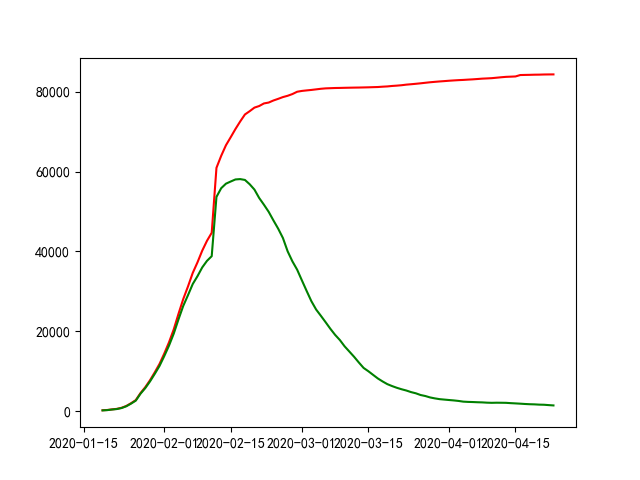
\includegraphics[width=0.45\textwidth]{plot1.png}
                    \caption{原始数据}
                    \label{plot1}
                \end{figure}

                \begin{figure}[H]
                    \centering
                    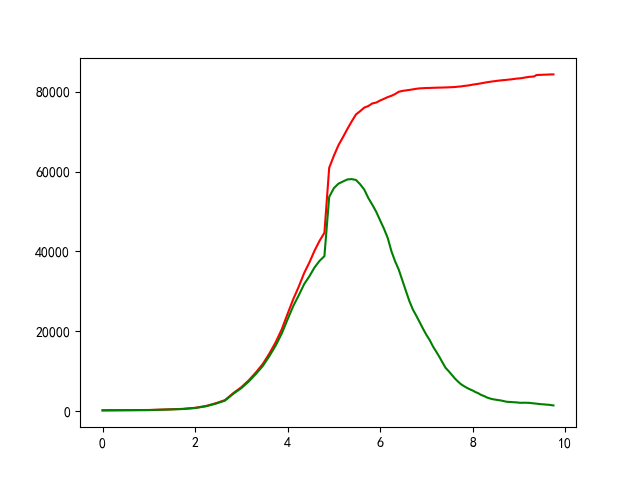
\includegraphics[width=0.45\textwidth]{plot2.png}
                    \caption{变换后的数据$y-\sqrt{x}$}
                    \label{plot2}
                \end{figure}
            \subsection{进行曲线拟合}
                如公式(\ref{z5})所示,我们需要对数据取对数,然后再进行拟合,我们对数据进行变换得到$\ln{y}-x$的图像,然后通过最小二乘法的相关程序进行拟合,拟合曲线如图\ref{plot3}的蓝色曲线所示。

                \begin{figure}[H]
                    \centering
                    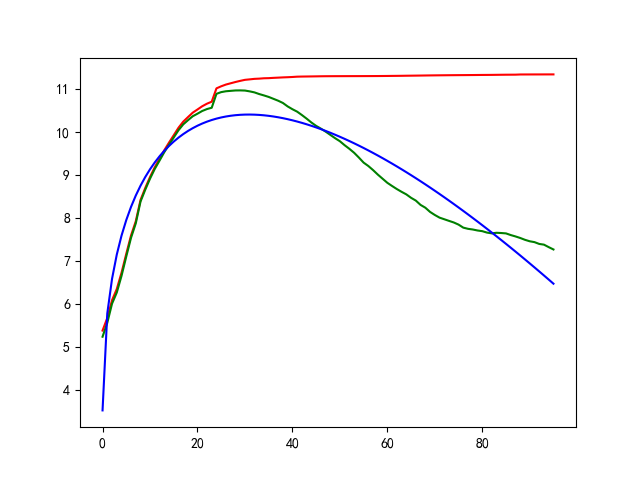
\includegraphics[width=0.45\textwidth]{plot3.png}
                    \caption{变换后的数据$\ln{y}-x$以及拟合曲线。}
                    \label{plot3}
                \end{figure}

                经过程序计算后,三个参数分别为$a=-0.22353727,b=2.48135593,c=3.52180996$,代入公式(\ref{z6})后,解得三个参数分别为$\sigma=2.1150713,\mu=5.5502063,k=8.0882235{\times}10^{14}(e^{34.236})$。

                代回公式(\ref{z4}),可得$y-x$大致符合公式(\ref{z7}),计算得到数据的残差和$\parallel\delta\parallel^2=8.25{\times}10^9$

                \begin{equation}
                    y=8.0882235{\times}10^{14}e^{-\frac{(\sqrt{x}-5.5502063)^2}{2.1150713^2}}
                    \label{z7}
                \end{equation}

                拟合后的曲线如图(\ref{plot4})所示,发现拟合的效果并不是很好,分析得出在$\ln{y}-x$的关系下进行最小二乘法的拟合会导致错误的情况发生。

                \begin{figure}[H]
                    \centering
                    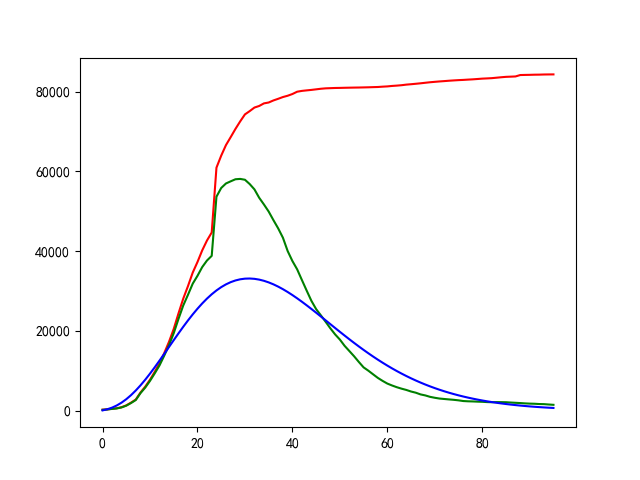
\includegraphics[width=0.45\textwidth]{plot4.png}
                    \caption{拟合曲线}
                    \label{plot4}
                \end{figure}

            \subsection{曲线拟合的改进方法}
                从之前的拟合过程可以看出,对$x-\ln{y}$进行拟合的效果并不是很好。因为在$0$附近,源数据点的波动将会通过$\ln{y}$放大,过多的噪声放大将会导致误差变大,甚至造成错误的结果。

                因此,在对曲线拟合进行优化时,可以设置一个阈值$Th$,当$y_{i}<Th$时,忽略该数据点。我们将阈值$Th$设置成$e^{9}$,即舍去$\ln{y_{i}}<9$的数据点。

                重新进行之前的曲线拟合后,得到的数据如图\ref{plot5},得到的三个参数分别是$a=-0.35241579,b=3.844773333,c=0.32331052$,这组数据相对于没有筛选的那组数据更加贴近原曲线,但是最高峰任然不是重合的。此时残差和$\parallel\delta\parallel^2=9.38{\times}10^8$

                \begin{figure}[H]
                    \centering
                    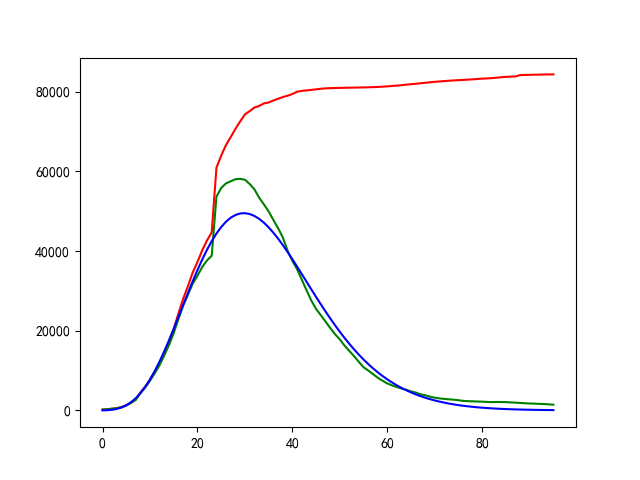
\includegraphics[width=0.45\textwidth]{plot5}
                    \caption{设置阈值$e^8$后的拟合曲线}
                    \label{plot5}
                \end{figure}

                之后再把阈值$Th$设置成$e^{9}$,在进行拟合,得到的图如图\ref{plot6}所示,其残差和$\parallel\delta\parallel=4.47{\times}10^8$,相对于上一组值曲线拟合的更好,计算得出$a=-0.35241579,b=3.844773333,c=0.32331052$,代入公式(\ref{z6})后,解得三个参数分别为$\sigma=1.5648762,\mu=5.5502063,k=2.050057831714{\times}10^{12}$。并得到满足的关系式如公式(\ref{z8})。

                \begin{equation}
                    y=8.0882235{\times}10^{14}e^{-\frac{(\sqrt{x}-5.5502063)^2}{2.1150713^2}}
                    \label{z8}
                \end{equation}

                \begin{figure}[H]
                    \centering
                    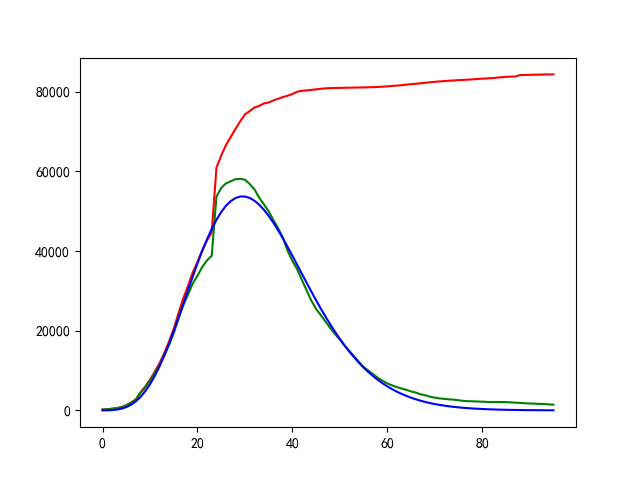
\includegraphics[width=0.45\textwidth]{plot6}
                    \caption{设置阈值$e^9$后的拟合曲线}
                    \label{plot6}
                \end{figure}
            \subsection{$Re(t)$的曲线}
                之前我们我们从正态分布出发,尝试对曲线进行拟合,得到了公式(\ref{z8}),我们对原始公式(\ref{z4})求导,可以得到下列公式,然后代入公式(\ref{z1}),可以得到$Re(t)$。

                \begin{equation}
                    \frac{di(t)}{dt}=-\frac{k(\sqrt{t}-\mu)}{\sigma^2\sqrt{t}}e^{-\frac{(\sqrt{t}-\mu)^2}{\sigma^2}}
                \end{equation}

                \begin{equation}
                    Re(t)=\frac{di(t)}{i(t)dt}+1=1-\frac{(\sqrt{t}-\mu)}{\sigma^2\sqrt{t}}{\quad}(t>0)
                    \label{z10}
                \end{equation}
                
                然后依据公式(\ref{z1}),并使用$i(t+dt)-i(t)$代替$dt$,可以得到下面的公式。

                \begin{equation}
                    Re^{*}(t)=\frac{i(t+dt)-i(t)}{i(t)dt}=\frac{{\Delta}i(t)}{i(t){\Delta}t}
                    \label{z11}
                \end{equation}

                我们用公式(\ref{z10})计算拟合的曲线,用公式(\ref{z11})计算实际数据,曲线如图所示,其中$Re(t)$为红色曲线,$Re_{*}(t)$为绿色曲线。发现两条曲线的拟合度并不是很好。我们观察绿色曲线发现,在疫情的前期,$Re{\approx}1.5$,到了后期$Re{\approx}0.95$,说明在现在,疫情还处于缓慢减退的阶段,因此现在还不可以放松警惕。

                \begin{figure}[H]
                    \centering
                    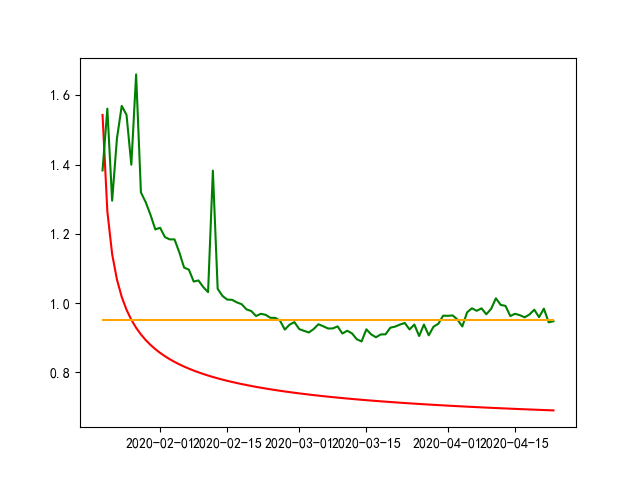
\includegraphics[width=0.45\textwidth]{plot8.png}
                    \caption{$Re(t)$和$Re^{*}(t)$曲线}
                    \label{plot8}
                \end{figure}

        \section{结果分析}
            \subsection{常用的传染病模型}
                这次传染病有潜伏期,而且患者在潜伏期内页仍然有传染性。传染病模型可以在一定程度上预测未来疫情的走势。

                比较适合这次疫情的传染病模型是\textbf{SEIR模型},在这个模型中,同一类型的人群是均质的,即并没有考虑\textbf{超级传播者}存在的可能性\cite{seir}。

                在\textbf{SEIR模型}中,$r_{1}$为感染者平均在$dt$的时间内接触的易感者人数,$\beta_{1}$为感染者传染的概率。$r_{2}$为潜伏者平均在$dt$的时间内接触的易感者人数,$\beta_{2}$为潜伏者传染的概率。$\sigma$为潜伏者转变成感染者的概率,$\gamma$为感染者转变成康复者的概率,$N$为人群的数量。基于此,我们可以得到下述微分方程,将其微分方程转化成\textbf{等价的动力系统},设置好初值不断迭代便能得到四种人群数量的变化曲线。

                \begin{gather}
                    \frac{dS}{dt}=-\frac{r_1{\beta}_1IS}{N}-\frac{r_2{\beta}_2ES}{N} \notag \\
                    \frac{dE}{dt}=\frac{r_1{\beta}_1IS}{N}-{\alpha}E+\frac{r_2{\beta}_2ES}{N} \notag \\
                    \frac{dI}{dt}={\alpha}E-{\gamma}I \notag \\
                    \frac{dR}{dt}={\gamma}I
                \end{gather}

                图(\ref{plot9})为参数$r_1=r_2=20,{\beta}_1={\beta}_2=0.03,\alpha=\gamma=0.1$的模拟情况,可以发现,这个模型除了在疫情后期,能够较好的反映疫情的发展情况。

                \begin{figure}[H]
                    \centering
                    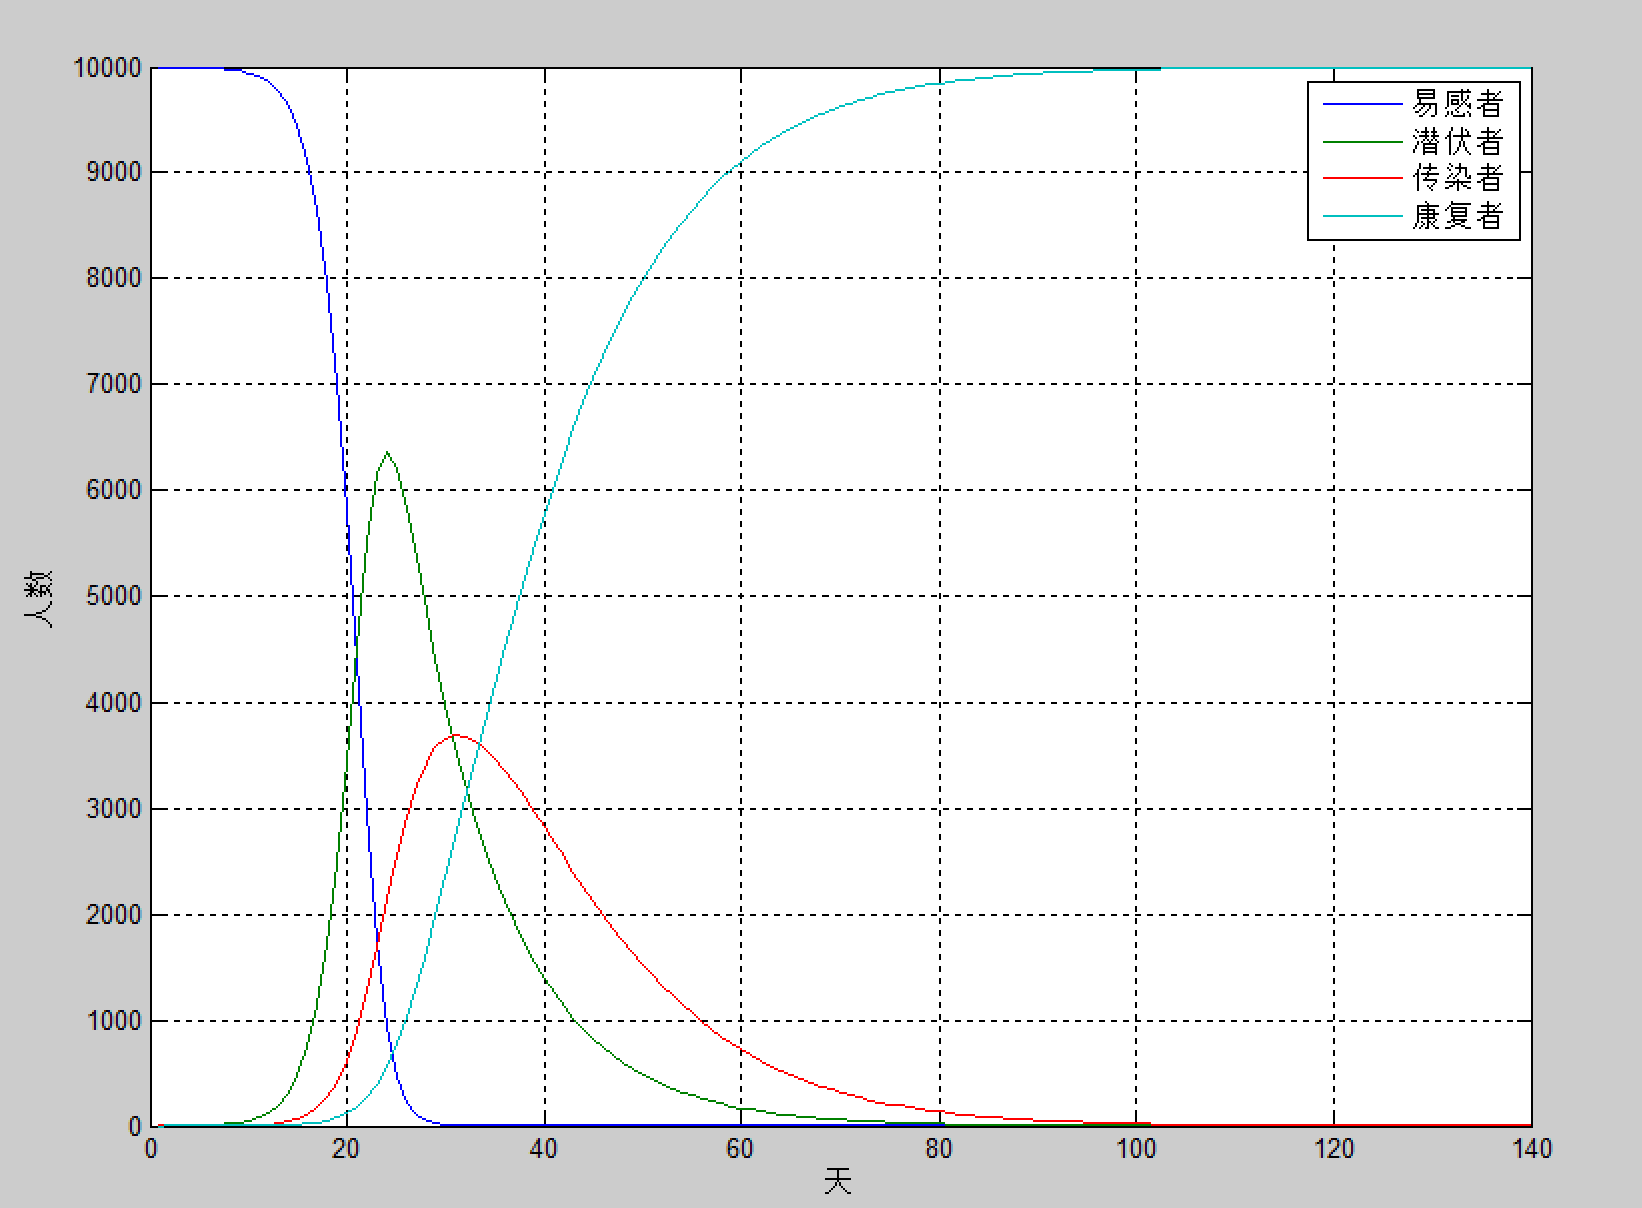
\includegraphics[width=0.45\textwidth]{plot9.png}
                    \caption{SEIR模型模拟情况}
                    \label{plot9}
                \end{figure}
            \subsection{最小二乘法的适应性}
                在\textbf{SEIR}模型中,由于微分方程比较复杂,在四个关系中隐含了四种人群满足的关系,但是由于方程复杂,无法求出解析式,因此只能通过猜测的方式去选择比较合适的函数进行拟合。在拟合的过程中,发现数据与曲线拟合的较好,但是这种拟合只是全局性。在这个例子中,拟合函数在接近$0$的数据附近表现并不是很好。

                而且,将$y$转化成$\ln{y}$容易导致误差放大的现象,使曲线更加贴近较小的数据,因此,最小二乘法适合于两者的函数关系比较简单或者具有确切关系的场合。

    \end{multicols}
    
    % \begin{figure}[H]
    %     \centering
    %     \subfigure[场景1]{
    %         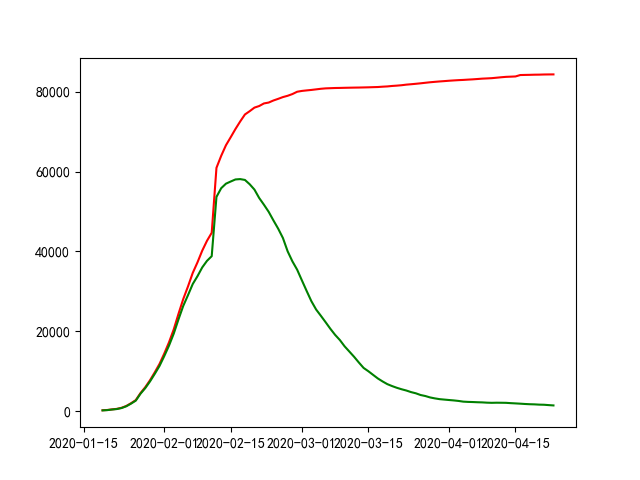
\includegraphics[width=0.45\textwidth]{plot1.png}
    %     }
    %     \subfigure[场景2]{
    %         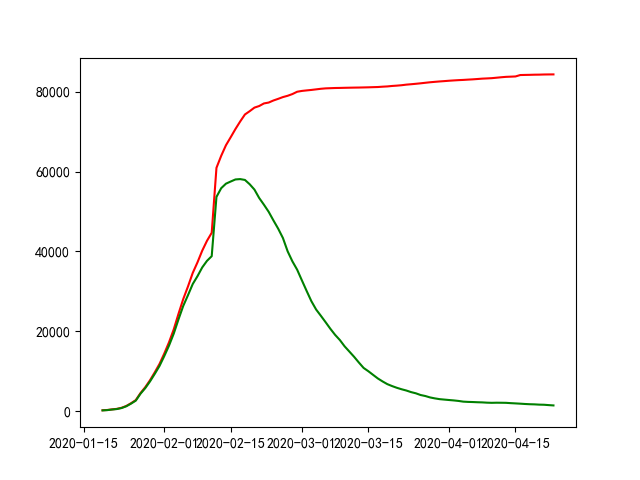
\includegraphics[width=0.45\textwidth]{plot1.png}
    %     }
    %     \caption{数据图}
    %     \label{}
    % \end{figure}

    \bibliographystyle{plain}
    \bibliography{spectral} 
    \begin{thebibliography}{1}
        \bibitem{model1}
        数据来源:中国政府网

        \bibitem{r0}
        少年游(知乎用户)
        \newblock{科普 | 基本传染数R0}
        \newblock{zhuanlan.zhihu.com/p/104128326}

        % 第一行作者;第二行文章标题;第三行杂志和页码
        \bibitem{seir}
        qwe14789cn(知乎用户)
        \newblock{在家宅着也能抵抗肺炎!玩一玩SEIR传染病模型}
        \newblock{zhuanlan.zhihu.com/p/104268573?night=1}

    \end{thebibliography}

\end{document}